\documentclass{article}
\usepackage[utf8]{inputenc}

\title{Deep Learning Classification Project MGI Vlasakker Zurcher}
\author{Raphael Zürcher \& Robert van de Vlasakker}
\date{April 2021}

\usepackage{natbib}
\usepackage{graphicx}
\usepackage[colorlinks, allcolors=blue]{hyperref}
\graphicspath{{figures/}}

\begin{document}

\maketitle

\section{Introduction}
In computer vision, deep learning is often used to automate tasks and accurately predict objects on remote sensing data. Deep learning used in Remote sensing usually can be divided into CNN and RNN application. CNN's are architectured of multi layer with convolutional layers and fully connected layers including activation functions and pooling, whereas RNN's recycles the output from previous time steps and are rather used for sequential data \citep{campos2020understanding}. In this paper, a CNN method is followed for single image classification with a single label approach and a multi label approach. We compare ResNet34, a residual neural network with our own simpler CNN model. Further, we compare the mean and none method in the binary cross entropy loss within the ResNet34 model implementation. The two methods are applied when representation of classes are heterogeneous. The used UC Merced dataset consists of 2100 images and are labeled \cite{yang2010bag}. Further, Pytorch provides a pretrained option, which allows to mitigate the training time for own datasets, which was done in this case for the imported ResNet34 model. Usually, the training for deeper networks is harder, but the deeper the CNN, the better the performance, though stagnates or degrades after a certain depth. This vanishing gradient is solved by the residual neural networks \citep{he2016deep}. 



\section{Methods}
\subsection{Single Label Classification}
\textbf{Data Loading}.
For the single label classification we used the folder names that contain the images as class label, e.g. if a image is located in the folder 'Airplane' the label for the image would be 'Airplane'.
There are 21 different image folder, so the total amount of classes would be 21.
The data is loaded data with ImageFolder() loader provided by Pytorch.
We wrote two custom function that where both inserted into the ImageFolder().
The first one was a function that reshapes the image to 256 by 256 and then transforms the PIL image to a tensor.
The second one was a small function that one hot encodes all the class labels. 
The data has been split with the utility tool random\_split().
We used 80\% for training (1680 samples) and 20\% for testing (420 samples).
While it is possible to calculate the optimal batch size with \(Max Batch = GPU memory  / 4 / (Tensor Size + Trainable Parameters)\), we use an arbitrary value of 128.
We are working on Google Colab and we do not know how much GPU memory is located to our Jupyter Notebook.
A batch size of 128 is also used because to the power of 2 generally works better \citep{DBLP:journals/corr/KeskarMNST16}.
The result of loading a single batch is a tensor of [128, 3, 256, 256].
\\ % newline

\noindent
\textbf{Model}. 
For the single label classification we used a pretrained ResNet model \citep{he2016deep}. 
We changed the last linear layer of the pretrained ResNet model to have 21 classes, instead of the original 1000.
Because we one hot encoded the the label classes we also added a final softmax (nn.Softmax()) layer.
This will squeeze all the predicted classes to have a value between zero and one, with a total of one.
The class with the highest value (theoretically 1 would be perfect), will be the image label.
With the training of the model we set all the parameters to true, because the parameters of the ResNet model are optimized for ImageNet (SOURCE).
We could also have downloaded a model that was trained on the UCM dataset, changed the linear output to match our amount of classes (if this was even necessary with the same dataset) and added the softmax layer.
In this case we would only have to train the last two layers.




\subsection{Multi Label Classification}
\textbf{Data Loading}
The data set contain 2100 RGB images with a resolution of 256 by 256 and a label file with the image name and their corresponding labels with 17 different classes in the case of multi label prediction.
The data set consists of a CVS file and a folder containing different folder (named after their class) containing the images.
We created a Data Class for the image data set using Pytorch. 
The Data Class takes to input variables: the image location folder and the CVS file contain the image labels.
Inside the data class the image location folder is used to read all the image locations.
These locations are all saved in a list and the list is sorted alphabetically so that is matched the CSV label list.
The CVS file is opened as a Pandas data frame and the list containing the image locations is added to the data frame as a new column.
Next, both the image and their corresponding label are loaded as a tensor.
The image is first transformed to a 256 by 256 tensor just in case. 
Finally, the Data Class returns both tensors.
\\

\noindent
\textbf{Models}.
We use two models in this project; a pretrained ResNet34 model with adapted linear layer and output layer and a new model build from scratch.
The last output layer of the ResNet has been adapted to match the amount of classes in our dataset, nn.linear(512, 17).
A final sigmoid layer has been added to the linear layer to make sure that a prediction between zero and one is returned for each of the classes. 
The final sigmoid function is added to the ResNet34 to get prediction values between 0 (not certain) and 1 (very certain) for each of the 17 classes. 
Our own implementation is a model build from scratch.
It uses the example model of the Pytorch. 
We use four different convolutional layers to extract information from the image. 
The dropout layer are added just for testing.
There are two maxpool layers present to reduce the amount of parameters in the model.
The linear layers are present to reduce the tensor output to have a size of 17 (equal to the amount of classes).
Finally, the sigmoid activation function is added to squeeze every value between zero and one, so for every image every class gets a prediction value.
We used a threshold value of 0.5 to determine if a class prediction is high enough.

\section{Implementation}
%? COLAB CODE?

\section{Results}
\section{Discussion}
\section{Conclusion}
\begin{figure}
    \centering
    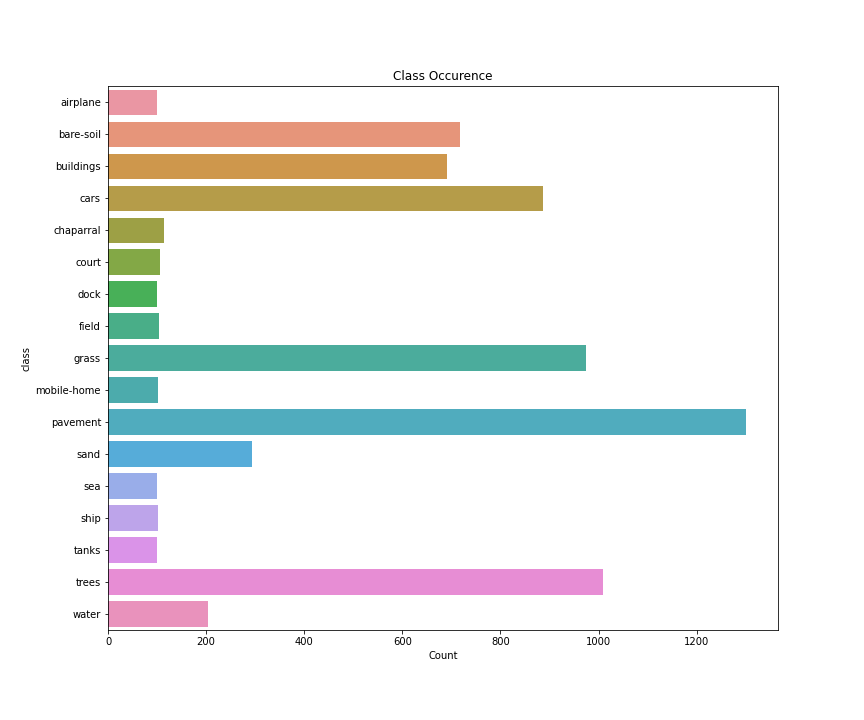
\includegraphics[width=1\textwidth]{classes.png}
    \caption{class representations}
    \label{fig:classes}
\end{figure}

\begin{figure}
    \centering
    
\includegraphics[width=1\textwidth]{train_picture_w_labels.png}
    \caption{image training with labels}
    \label{fig:trainpicture}
\end{figure}



\bibliographystyle{plain}
\bibliography{references}


\end{document}

- compare resnet34 with own model
- compare reduction none (sum; mean) > overrepresented classes 
- why adapted resnet
- Sigmoid --> because we need multiple classes output
- Adapted resnet to have 17 output classes
- Talk about the class distribution
- adapt epochs > time consumption